\chapter{Cellular Network}

\section{Multiple Access}

\textbf{Frequency Division Multiple Access (FDMA)}\\[0.5em]
It assigns a unique frequency channel to each user for the duration of the call. A guard band is needed to prevent interference between adjacent channels. Mobile terminals operate with dedicated uplink and downlink frequencies, but since frequency spectrum is limited and valuable, efficient usage is critical—leading to the exploration of technologies like cognitive radio.

\textbf{Time Division Multiple Access (TDMA)}\\[0.5em]
It divides time into slots, where each user transmits only during their assigned time slot, avoiding contention. Unlike WiFi's CSMA, TDMA ensures no overlap among users. A guard time is necessary to account for different signal arrival times from users at varying distances from the base station.

\textbf{Code Division Multiple Access (CDMA)}\\[0.5em]
It allows all users to share the same frequency band simultaneously by assigning unique orthogonal codes to each. Data is spread over a wider bandwidth using these codes, enabling multiple transmissions to coexist without interference due to code separation.

\section{GSM (Global System for Mobile Communications)}

\begin{figure}[H]
   \centering
   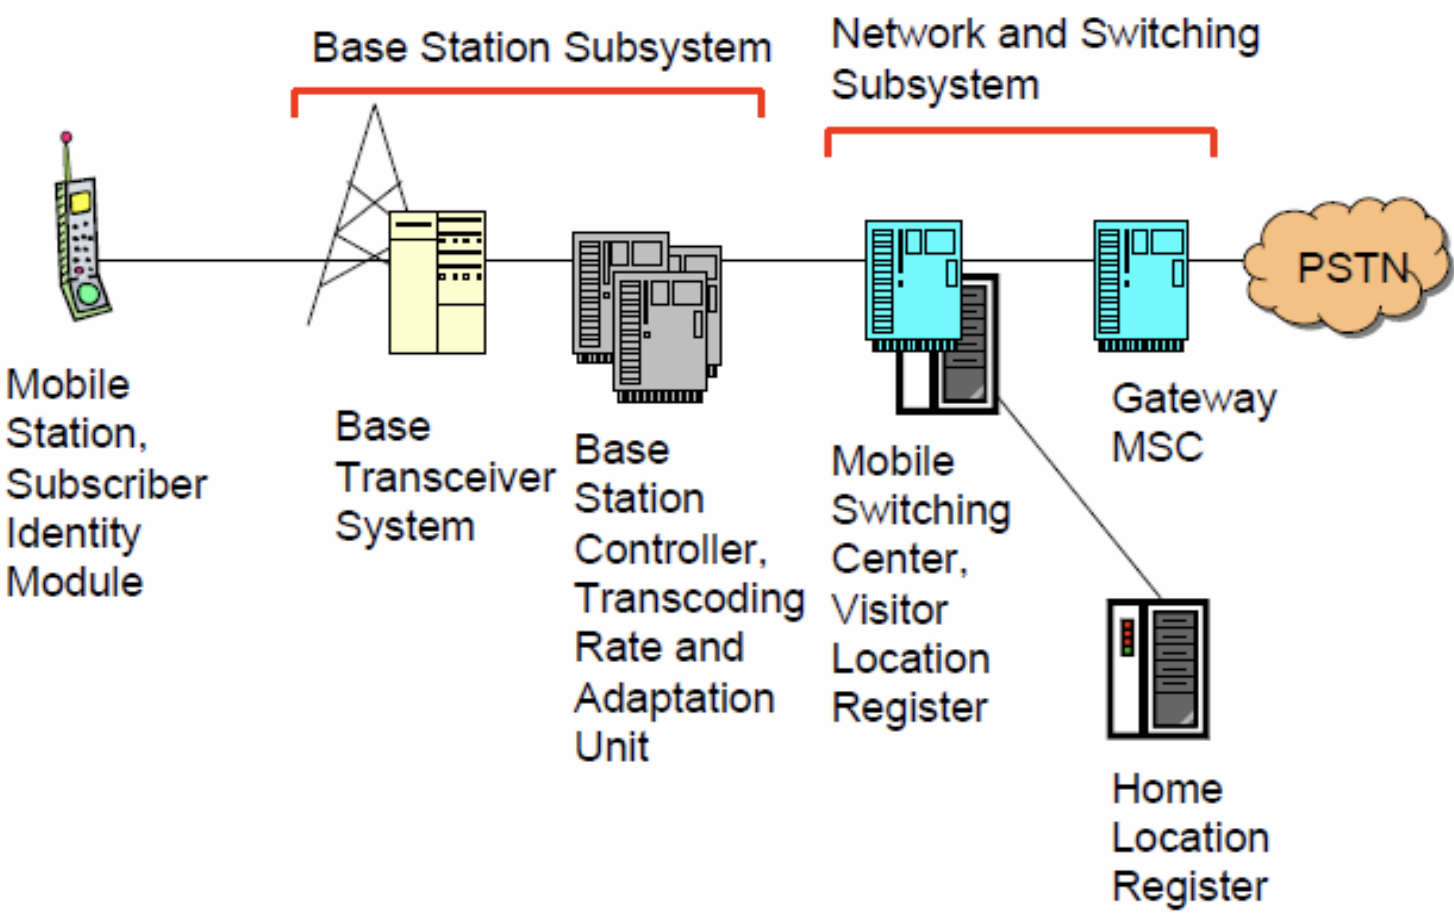
\includegraphics[width=0.6\textwidth]{figures/GSM.png}
\end{figure}

\section{Cellular Network Components}

\subsection{Mobile Station (MS)}
The mobile station consists of a mobile device (like a smartphone) and a SIM card. The SIM card contains the International Mobile Subscriber Identity (IMSI) and Personal Identification Number (PIN), which uniquely identifies the user on the network.

\subsection{Mobile Switching Center (MSC)}
The MSC is a central component in a cellular network that connects calls by establishing a path between the calling and receiving parties. It manages call routing, handovers, mobility management, and collecting billing information.
% The MSC also interfaces with other networks, such as the Public Switched Telephone Network (PSTN) for voice calls.

\subsection{Base Station Subsystem (BSS)}
The BSS consists of the \rgbO{Base Transceiver Station (BTS)} and \rgbO{Base Station Controller (BSC)}. The BTS handles radio communication with mobile devices. It contains the equipment for transmitting and receiving of radio signals (transceivers), antennas, and equipment for encrypting and decrypting communications with the BSC. BSC manages multiple BTSs, controlling radio resources, handovers, and frequency allocation.

\section{Handoff (Handover)}
Within a BSS, the BSC, which knows the current radio link configuration (including feedbacks from the MS), prepares an available channel in the new BTS. Then the MS is told to switch over to the new BTS. This is called a hard handoff. In a soft handoff, the MS is connected to two BTSes simultaneously.